\section{Struktur Derivasi dan Ambiguitas}

\subsection{Leftmost vs Rightmost Derivation}
\textit{Leftmost derivation} (LD) selalu mengganti non-terminal paling kiri, sering digunakan pada top-down parser. Sebaliknya, \textit{Rightmost derivation} (RD) mengganti non-terminal paling kanan, umum pada bottom-up parser.

\subsection{Ambiguitas Grammar}
Grammar disebut ambigu jika satu input dapat menghasilkan lebih dari satu \textit{parse tree}. Hal ini berbahaya karena dapat menyebabkan salah interpretasi logika program (misal: urutan operasi aritmatika).

\begin{figure}[!htbp]
    \centering
    \adjustbox{max width=0.8\textwidth,center}{%
    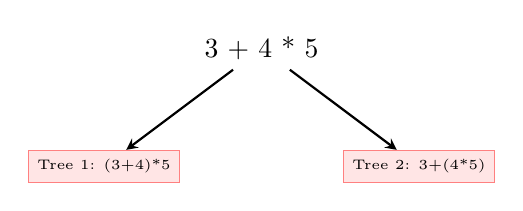
\begin{tikzpicture}[
        tree/.style={rectangle, draw=red!50, fill=red!10, font=\tiny, align=center},
        arrow/.style={->, >=stealth, thick}
    ]
    \node (in) at (0,0) {3 + 4 * 5};
    \node[tree] (t1) at (-2,-1.5) {Tree 1: (3+4)*5};
    \node[tree] (t2) at (2,-1.5) {Tree 2: 3+(4*5)};
    \draw[arrow] (in) -- (t1);
    \draw[arrow] (in) -- (t2);
    \end{tikzpicture}%
    }
    \caption{Ilustrasi ambiguitas grammar}
\end{figure}
